%\documentclass[ckj,dvipdfmx]{beamer}
\documentclass[ckj,dvipdfmx]{beamer}
\usepackage{etex}
%\usetheme{Warsaw}
\usetheme{Malmoe}
%\usetheme{AnnArbor}
%\usetheme{Hannover}
%\usetheme{Bergen}
%\usetheme{Berlin}
%\usetheme{Singapore}
%\usetheme{Montpellier}
%\usetheme{Pittsburgh}
\usepackage{graphicx}
\usepackage{latexsym,amssymb}
\usepackage{amsthm}
%\usepackage{epsbox}
%\usepackage{multirow}
%\usepackage{fancybox}
\usepackage{tikz}
\usetikzlibrary{calc}
\usepackage{fancyvrb}
%\usepackage{listings}
\usepackage{tabularx}
%\usepackage{pstricks,pst-node,pst-tree}
%\usepackage{multimedia}
%\usepackage{pstricks,pst-node,pst-tree}
%\usepackage{pst-all}
%\include{prooftree}
%\lstloadlanguages{pascal}
\usepackage{mathrsfs}
\renewcommand{\kanjifamilydefault}{\gtdefault}
\renewcommand{\familydefault}{\sfdefault}

\newcommand{\greentext}[1]{{\color[rgb]{0,0.5,0}{#1}}}
\newcommand{\redtext}[1]{{\color[rgb]{0.8,0,0}{#1}}}
\newcommand{\bluetext}[1]{{\color[rgb]{0,0,0.8}{#1}}}

\newcommand{\tuple}[1]{\langle{#1}\rangle}

\newcommand{\First}{\mathsf{First}_1}
\newcommand{\Follow}{\mathsf{Follow}_1}

%%pdt simulation

\newcommand{\pdtline}[6]{%
    \uncover<#6->{
        \node at (${#5}*(0,-.3)+(0,.3)$) {$\vdash$};%
        \node at (${#5}*(0,-.3)+(1.5,.3)$) {\parbox{12em}{(#1,}};%
        \node at (${#5}*(0,-.3)+(4.5,.3)$) {\parbox{10em}{#2,}};%
        \node at (${#5}*(0,-.3)+(5.7,.3)$) {\parbox{10em}{#3)}};%
        \node at (${#5}*(0,-.3)+(8,.3)$) {\parbox{20em}{#4}};%
    }
}

\newcommand{\initpdtline}[6]{%
    \uncover<#6->{
        \node at (${#5}*(0,-.3)+(1.5,.3)$) {\parbox{12em}{(#1,}};%
        \node at (${#5}*(0,-.3)+(4.5,.3)$) {\parbox{10em}{#2,}};%
        \node at (${#5}*(0,-.3)+(5.7,.3)$) {\parbox{10em}{#3)}};%
        \node at (${#5}*(0,-.3)+(8,.3)$) {\parbox{20em}{#4}};%
    }
}

\newtheorem{Def}{定義}
\newtheorem{Lem}{補題}
\newtheorem{Thm}{定理}
\newtheorem{Prop}{命題}

\definecolor{lightlightgrey}{rgb}{0.95,0.95,0.95}
\definecolor{darkgreen}{rgb}{0,0.64,0}

\newcommand{\vdom}{\underline{\gg}}
\newcommand{\svdom}{\gg}

\newcommand{\ttpl}{\texttt{+}}
\newcommand{\ttsb}{\texttt{-}}
\newcommand{\ttmu}{\texttt{*}}
\newcommand{\ttdv}{\texttt{/}}
%\include{cmacros}

%\newcommand{\greentext}[1]{{\color[rgb]{0,0.5,0}{#1}}}
%\newcommand{\redtext}[1]{{\color[rgb]{0.8,0,0}{#1}}}

\newcommand{\lecturedate}{2026/11/27}

%\cornersize{0.25}
\graphicspath{{figs261127/}}

\setbeamertemplate{frametitle}[default][center]
\setbeamertemplate{footline}{\hfill
コンパイラ\quad\lecturedate
\hfill\insertframenumber/\inserttotalframenumber\hspace*{1zw}}
\newcounter{coffee}
\setbeamercovered{transparent=10}
\title{コンパイラ(15)}
\date{\lecturedate}
\begin{document}
\frame{\titlepage}
\section{レジスタ割当}
\subsection{弦グラフの彩色}
\begin{frame}
    \frametitle{弦グラフ}
    \begin{Def}
        無向グラフにおいて，長さ４以上の閉路に対して，弦となる辺が存在する．
        弦：閉路上で隣接しない頂点を結ぶ辺
    \end{Def}
    \vspace*{10pt}
    \begin{center}
        \begin{tabularx}{.6\linewidth}{XX}
            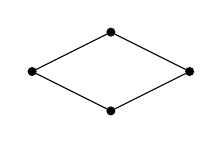
\begin{tikzpicture}
                \node[draw,circle,inner sep=1pt,fill=black] (N0) at (0,0) {};
                \node[draw,circle,inner sep=1pt,fill=black] (N1) at (1,0.5) {};
                \node[draw,circle,inner sep=1pt,fill=black] (N2) at (1,-0.5) {};
                \node[draw,circle,inner sep=1pt,fill=black] (N3) at (2,0) {};
                \path[-] (N0) edge (N1) (N1) edge (N3) (N0) edge (N2) (N2) edge (N3);
            \end{tikzpicture}
                    &
            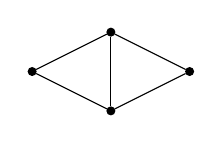
\begin{tikzpicture}
                \node[draw,circle,inner sep=1pt,fill=black] (N0) at (0,0) {};
                \node[draw,circle,inner sep=1pt,fill=black] (N1) at (1,0.5) {};
                \node[draw,circle,inner sep=1pt,fill=black] (N2) at (1,-0.5) {};
                \node[draw,circle,inner sep=1pt,fill=black] (N3) at (2,0) {};
                \path[-] (N0) edge (N1) (N1) edge (N3) (N0) edge (N2) (N2) edge (N3) (N1) edge (N2);
            \end{tikzpicture} \\
            弦グラフでない & 弦グラフ
        \end{tabularx}
    \end{center}

    頂点消去：隣接頂点との辺をすべて消去し，隣接頂点間が互いに隣接になるように辺を加える．(Fill-in辺)

    \vspace*{10pt}

    \greentext{弦グラフ：Fill-in辺が必要ないように頂点を消去することが可能}

    \vspace*{10pt}

    Fill-in辺なく消去する頂点の順番＝完全消去順序(PEO)\\
    計算量：$\mathcal{O}(|V|+|E|)$
\end{frame}

\begin{frame}
    \frametitle{完全消去順序(PEO)}
\only<1>{
\begin{center}
        \begin{tabular}{cccc}
            & 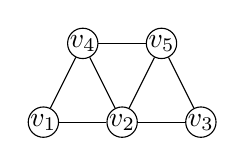
\begin{tikzpicture}
                \node[draw,circle,inner sep=0pt] (V1) at (0,0) {$v_1$};
                \node[draw,circle,inner sep=0pt] (V2) at (1,0) {$v_2$};
                \node[draw,circle,inner sep=0pt] (V3) at (2,0) {$v_3$};
                \node[draw,circle,inner sep=0pt] (V4) at (0.5,1) {$v_4$};
                \node[draw,circle,inner sep=0pt] (V5) at (1.5,1) {$v_5$};
                \path[-] (V1) edge (V2) (V2) edge (V3) (V1) edge (V4) (V4) edge (V2)
                (V4) edge (V5) (V2) edge (V5) (V5) edge (V3);
            \end{tikzpicture}
            & $v_3$を消去$\Rightarrow$ &
            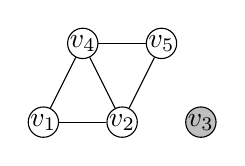
\begin{tikzpicture}
                \node[draw,circle,inner sep=0pt] (V1) at (0,0) {$v_1$};
                \node[draw,circle,inner sep=0pt] (V2) at (1,0) {$v_2$};
                \node[draw,circle,inner sep=0pt,fill=gray!50] (V3) at (2,0) {$v_3$};
                \node[draw,circle,inner sep=0pt] (V4) at (0.5,1) {$v_4$};
                \node[draw,circle,inner sep=0pt] (V5) at (1.5,1) {$v_5$};
                \path[-] (V1) edge (V2) (V1) edge (V4) (V4) edge (V2)
                (V4) edge (V5) (V2) edge (V5);
            \end{tikzpicture}                                                                            \\[10pt]
            $v_5$を消去$\Rightarrow$                                                 &
            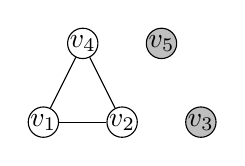
\begin{tikzpicture}
                \node[draw,circle,inner sep=0pt] (V1) at (0,0) {$v_1$};
                \node[draw,circle,inner sep=0pt] (V2) at (1,0) {$v_2$};
                \node[draw,circle,inner sep=0pt,fill=gray!50] (V3) at (2,0) {$v_3$};
                \node[draw,circle,inner sep=0pt] (V4) at (0.5,1) {$v_4$};
                \node[draw,circle,inner sep=0pt,fill=gray!50] (V5) at (1.5,1) {$v_5$};
                \path[-] (V1) edge (V2) (V1) edge (V4) (V4) edge (V2);
            \end{tikzpicture} &
            $v_4$を消去$\Rightarrow$                                                 &
            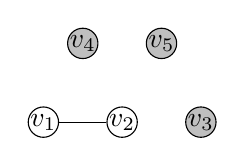
\begin{tikzpicture}
                \node[draw,circle,inner sep=0pt] (V1) at (0,0) {$v_1$};
                \node[draw,circle,inner sep=0pt] (V2) at (1,0) {$v_2$};
                \node[draw,circle,inner sep=0pt,fill=gray!50] (V3) at (2,0) {$v_3$};
                \node[draw,circle,inner sep=0pt,fill=gray!50] (V4) at (0.5,1) {$v_4$};
                \node[draw,circle,inner sep=0pt,fill=gray!50] (V5) at (1.5,1) {$v_5$};
                \path[-] (V1) edge (V2);
            \end{tikzpicture}\\[10pt]
            $v_1$を消去$\Rightarrow$                                                 &
            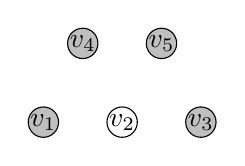
\begin{tikzpicture}
                \node[draw,circle,inner sep=0pt,fill=gray!50] (V1) at (0,0) {$v_1$};
                \node[draw,circle,inner sep=0pt] (V2) at (1,0) {$v_2$};
                \node[draw,circle,inner sep=0pt,fill=gray!50] (V3) at (2,0) {$v_3$};
                \node[draw,circle,inner sep=0pt,fill=gray!50] (V4) at (0.5,1) {$v_4$};
                \node[draw,circle,inner sep=0pt,fill=gray!50] (V5) at (1.5,1) {$v_5$};
            \end{tikzpicture} &
            $v_2$を消去$\Rightarrow$                                                 &
            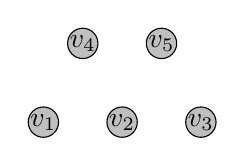
\begin{tikzpicture}
                \node[draw,circle,inner sep=0pt,fill=gray!50] (V1) at (0,0) {$v_1$};
                \node[draw,circle,inner sep=0pt,fill=gray!50] (V2) at (1,0) {$v_2$};
                \node[draw,circle,inner sep=0pt,fill=gray!50] (V3) at (2,0) {$v_3$};
                \node[draw,circle,inner sep=0pt,fill=gray!50] (V4) at (0.5,1) {$v_4$};
                \node[draw,circle,inner sep=0pt,fill=gray!50] (V5) at (1.5,1) {$v_5$};
            \end{tikzpicture}
        \end{tabular}\\[20pt]
        $v_3\rightarrow v_5\rightarrow v_4\rightarrow v_1\rightarrow v_2$は$PEO$
\end{center}
}
\only<2>{
\begin{center}
        \begin{tabular}{cccc}
            & 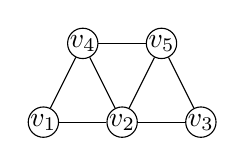
\begin{tikzpicture}
                \node[draw,circle,inner sep=0pt] (V1) at (0,0) {$v_1$};
                \node[draw,circle,inner sep=0pt] (V2) at (1,0) {$v_2$};
                \node[draw,circle,inner sep=0pt] (V3) at (2,0) {$v_3$};
                \node[draw,circle,inner sep=0pt] (V4) at (0.5,1) {$v_4$};
                \node[draw,circle,inner sep=0pt] (V5) at (1.5,1) {$v_5$};
                \path[-] (V1) edge (V2) (V2) edge (V3) (V1) edge (V4) (V4) edge (V2)
                (V4) edge (V5) (V2) edge (V5) (V5) edge (V3);
            \end{tikzpicture}
            & $v_2$を消去$\Rightarrow$ &
            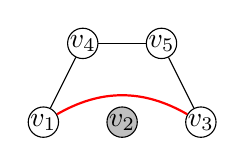
\begin{tikzpicture}
                \node[draw,circle,inner sep=0pt] (V1) at (0,0) {$v_1$};
                \node[draw,circle,inner sep=0pt,fill=gray!50] (V2) at (1,0) {$v_2$};
                \node[draw,circle,inner sep=0pt] (V3) at (2,0) {$v_3$};
                \node[draw,circle,inner sep=0pt] (V4) at (0.5,1) {$v_4$};
                \node[draw,circle,inner sep=0pt] (V5) at (1.5,1) {$v_5$};
                \path[-] (V1) edge (V4) (V4) edge (V5) (V5) edge (V3);
                \path[-,thick,color=red] (V1) edge [bend left] (V3);
            \end{tikzpicture}                                                                            \\[10pt]
            $v_3$を消去$\Rightarrow$                                                 &
            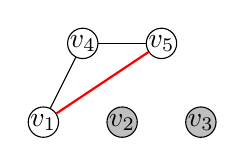
\begin{tikzpicture}
                \node[draw,circle,inner sep=0pt] (V1) at (0,0) {$v_1$};
                \node[draw,circle,inner sep=0pt,fill=gray!50] (V2) at (1,0) {$v_2$};
                \node[draw,circle,inner sep=0pt,fill=gray!50] (V3) at (2,0) {$v_3$};
                \node[draw,circle,inner sep=0pt] (V4) at (0.5,1) {$v_4$};
                \node[draw,circle,inner sep=0pt] (V5) at (1.5,1) {$v_5$};
                \path[-] (V1) edge (V4) (V4) edge (V5);
                \path[-,thick,color=red] (V1) edge (V5);
            \end{tikzpicture} &
            $v_1$を消去$\Rightarrow$                                                 &
            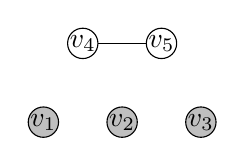
\begin{tikzpicture}
                \node[draw,circle,inner sep=0pt,fill=gray!50] (V1) at (0,0) {$v_1$};
                \node[draw,circle,inner sep=0pt,fill=gray!50] (V2) at (1,0) {$v_2$};
                \node[draw,circle,inner sep=0pt,fill=gray!50] (V3) at (2,0) {$v_3$};
                \node[draw,circle,inner sep=0pt] (V4) at (0.5,1) {$v_4$};
                \node[draw,circle,inner sep=0pt] (V5) at (1.5,1) {$v_5$};
                \path[-] (V4) edge (V5);
            \end{tikzpicture}\\[10pt]
            $v_5$を消去$\Rightarrow$                                                 &
            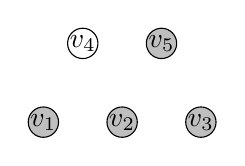
\begin{tikzpicture}
                \node[draw,circle,inner sep=0pt,fill=gray!50] (V1) at (0,0) {$v_1$};
                \node[draw,circle,inner sep=0pt,fill=gray!50] (V2) at (1,0) {$v_2$};
                \node[draw,circle,inner sep=0pt,fill=gray!50] (V3) at (2,0) {$v_3$};
                \node[draw,circle,inner sep=0pt] (V4) at (0.5,1) {$v_4$};
                \node[draw,circle,inner sep=0pt,fill=gray!50] (V5) at (1.5,1) {$v_5$};
            \end{tikzpicture} &
            $v_4$を消去$\Rightarrow$                                                 &
            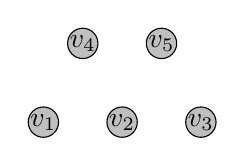
\begin{tikzpicture}
                \node[draw,circle,inner sep=0pt,fill=gray!50] (V1) at (0,0) {$v_1$};
                \node[draw,circle,inner sep=0pt,fill=gray!50] (V2) at (1,0) {$v_2$};
                \node[draw,circle,inner sep=0pt,fill=gray!50] (V3) at (2,0) {$v_3$};
                \node[draw,circle,inner sep=0pt,fill=gray!50] (V4) at (0.5,1) {$v_4$};
                \node[draw,circle,inner sep=0pt,fill=gray!50] (V5) at (1.5,1) {$v_5$};
            \end{tikzpicture}
        \end{tabular}\\[20pt]
        $v_2\rightarrow v_3\rightarrow v_1\rightarrow v_5\rightarrow v_4$は$PEO$でない (Fill-in辺が必要)
\end{center}
}
\end{frame}
\begin{frame}
    \frametitle{PEOによる彩色}
\begin{center}
        \begin{tabular}{cccc}
            & 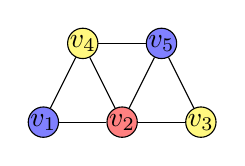
\begin{tikzpicture}
                \node[draw,circle,inner sep=0pt,fill=blue!50] (V1) at (0,0) {$v_1$};
                \node[draw,circle,inner sep=0pt,fill=red!50] (V2) at (1,0) {$v_2$};
                \node[draw,circle,inner sep=0pt,fill=yellow!50] (V3) at (2,0) {$v_3$};
                \node[draw,circle,inner sep=0pt,fill=yellow!50] (V4) at (0.5,1) {$v_4$};
                \node[draw,circle,inner sep=0pt,fill=blue!50] (V5) at (1.5,1) {$v_5$};
                \path[-] (V1) edge (V2) (V2) edge (V3) (V1) edge (V4) (V4) edge (V2)
                (V4) edge (V5) (V2) edge (V5) (V5) edge (V3);
            \end{tikzpicture}
            & $v_3$を彩色$\Leftarrow$ &
            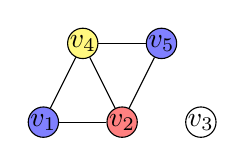
\begin{tikzpicture}
                \node[draw,circle,inner sep=0pt,fill=blue!50] (V1) at (0,0) {$v_1$};
                \node[draw,circle,inner sep=0pt,fill=red!50] (V2) at (1,0) {$v_2$};
                \node[draw,circle,inner sep=0pt] (V3) at (2,0) {$v_3$};
                \node[draw,circle,inner sep=0pt,fill=yellow!50] (V4) at (0.5,1) {$v_4$};
                \node[draw,circle,inner sep=0pt,fill=blue!50] (V5) at (1.5,1) {$v_5$};
                \path[-] (V1) edge (V2) (V1) edge (V4) (V4) edge (V2)
                (V4) edge (V5) (V2) edge (V5);
            \end{tikzpicture}                                                                            \\[10pt]
            $v_5$を彩色$\Leftarrow$                                                 &
            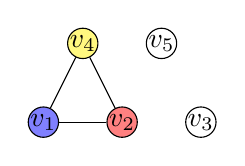
\begin{tikzpicture}
                \node[draw,circle,inner sep=0pt,fill=blue!50] (V1) at (0,0) {$v_1$};
                \node[draw,circle,inner sep=0pt,fill=red!50] (V2) at (1,0) {$v_2$};
                \node[draw,circle,inner sep=0pt] (V3) at (2,0) {$v_3$};
                \node[draw,circle,inner sep=0pt,fill=yellow!50] (V4) at (0.5,1) {$v_4$};
                \node[draw,circle,inner sep=0pt] (V5) at (1.5,1) {$v_5$};
                \path[-] (V1) edge (V2) (V1) edge (V4) (V4) edge (V2);
            \end{tikzpicture} &
            $v_4$を彩色$\Leftarrow$                                                 &
            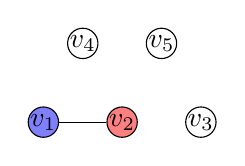
\begin{tikzpicture}
                \node[draw,circle,inner sep=0pt,fill=blue!50] (V1) at (0,0) {$v_1$};
                \node[draw,circle,inner sep=0pt,fill=red!50] (V2) at (1,0) {$v_2$};
                \node[draw,circle,inner sep=0pt] (V3) at (2,0) {$v_3$};
                \node[draw,circle,inner sep=0pt] (V4) at (0.5,1) {$v_4$};
                \node[draw,circle,inner sep=0pt] (V5) at (1.5,1) {$v_5$};
                \path[-] (V1) edge (V2);
            \end{tikzpicture}\\[10pt]
            $v_1$を彩色$\Leftarrow$                                                 &
            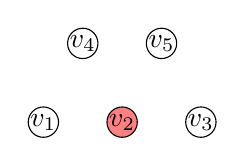
\begin{tikzpicture}
                \node[draw,circle,inner sep=0pt] (V1) at (0,0) {$v_1$};
                \node[draw,circle,inner sep=0pt,fill=red!50] (V2) at (1,0) {$v_2$};
                \node[draw,circle,inner sep=0pt] (V3) at (2,0) {$v_3$};
                \node[draw,circle,inner sep=0pt] (V4) at (0.5,1) {$v_4$};
                \node[draw,circle,inner sep=0pt] (V5) at (1.5,1) {$v_5$};
            \end{tikzpicture} &
            $v_2$を彩色$\Leftarrow$                                                 &
            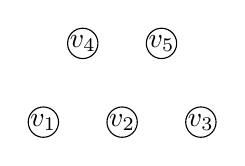
\begin{tikzpicture}
                \node[draw,circle,inner sep=0pt] (V1) at (0,0) {$v_1$};
                \node[draw,circle,inner sep=0pt] (V2) at (1,0) {$v_2$};
                \node[draw,circle,inner sep=0pt] (V3) at (2,0) {$v_3$};
                \node[draw,circle,inner sep=0pt] (V4) at (0.5,1) {$v_4$};
                \node[draw,circle,inner sep=0pt] (V5) at (1.5,1) {$v_5$};
            \end{tikzpicture}
        \end{tabular}\\[20pt]
        $v_2\rightarrow v_1\rightarrow v4\rightarrow v_5\rightarrow v_3$の順に彩色する
\end{center}
\end{frame}

\begin{frame}
\frametitle{弦グラフの彩色数}

グラフ$G=(V,E)$
\begin{list}{}{}
\item クリークのサイズ:$\omega(G)$
\item 彩色数(chromatic number):$\chi(G)$ \greentext{何色で彩色可能か？}
\end{list}
\begin{Prop}
$G$が弦グラフであるとき，$\omega(G)=\chi(G)$
\end{Prop}

\begin{Prop}
弦グラフ$G$は$\mathcal{O}(|V|+|E|)$で彩色可能である．
\end{Prop}
\end{frame}

\subsection{干渉グラフ}

\begin{frame}
\frametitle{SSA形式に対する変数の干渉グラフ}
$\varphi$関数を消去する前の$SSA$形式が対象\\
\greentext{$\varphi$関数消去後は定義が１箇所にならない}
\begin{Prop}
SSA形式における変数$v$の生存範囲は，支配木における連結部分木である．
\end{Prop}

SSA形式において，変数$v$が参照されるノードは$D_v$に支配される．
$v$が上書きされるまでは連結した部分木として$v$は生存する．

\end{frame}

\begin{frame}
\frametitle{例}
\begin{tabularx}{\linewidth}{m{.5\linewidth}m{.\linewidth}}
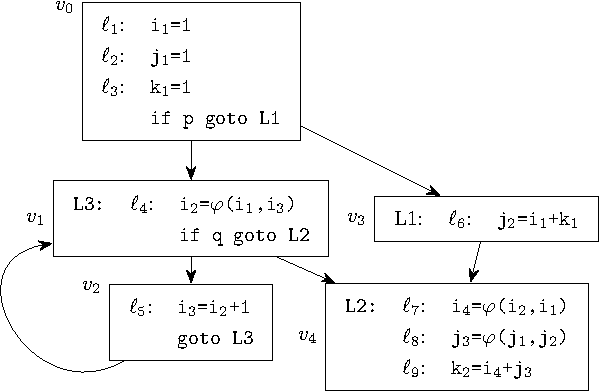
\includegraphics[scale=0.5]{figs261127/SSA-example4-SSA-crop.pdf}
&
{\small
\begin{tabular}{l|ll}
      & live-in & live-out\\\hline
$\ell_1$ &         & $\{i_1\}$\\
$\ell_2$ & $\{i_1\}$ & $\{i_1,j_1\}$\\
$\ell_3$ & $\{i_1,j_1\}$ & $\{i_1,j_1,k_1\}$\\
$\ell_4$ & $\{i_1,i_3,j_1\}$ & $\{i_2,j_1\}$\\
$\ell_5$ & $\{i_2,j_1\}$ & $\{i_3,j_1\}$\\
$\ell_6$ & $\{i_1,k_1\}$ & $\{i_1,j_2\}$ \\
$\ell_7$ & $\{i_1,i_2\}$ & $\{i_4\}$ \\
$\ell_8$ & $\{j_1,j_2\}$ & $\{j_3\}$ \\
$\ell_9$ & $\{i_4,j_3\}$ & $\{k_2\}$ \\
\end{tabular}}
\end{tabularx}

\vspace*{10pt}

\greentext{\small
$\mathsf{p}$, $\mathsf{q}$は更新されないのでここでは定数として扱う．
}
% \begin{center}
% \begin{tikzpicture}
% \node at (0,0) {$i_1$};\node[draw] (I11) at (0,-0.5) {$B_1$};\node[draw] (I12) at (0,-1.5) {$B_2$};\path[->] (I11) edge (I12);
% \node at (1,0) {$i_2$};\node[draw] (I21) at (1,-0.5) {$B_2$};\node[draw] (I22) at (1,-1.5) {$B_3$};\path[->] (I21) edge (I22);
% \node at (2,0) {$i_3$};\node[draw] (I31) at (2,-0.5) {$B_3$};
% \node at (3,0) {$i_4$};\node[draw] (I41) at (3,-0.5) {$B_5$};
% \node at (4,0) {$j_1$};\node[draw] (J11) at (4,-0.5) {$B_1$};\node[draw] (J12) at (4,-1.5) {$B_2$};\node[draw] (J13)at (4,-2.5) {$B_3$};\path[->] (J11) edge (J12) (J12) edge (J13);
% \node at (5,0) {$j_2$};\node[draw] (J21) at (5,-0.5) {$B_4$};
% \node at (6,0) {$j_3$};\node[draw] (J31) at (6,-0.5) {$B_5$};
% \node at (7,0) {$k_1$};\node[draw] (K11) at (7,-0.5) {$B_1$};\node[draw] (K12) at (7,-1.5) {$B_4$};\path[->] (K11) edge (K12);
% \node at (8,0) {$k_2$};\node at (8,-0.5) {$\varnothing$};
% \end{tikzpicture}
% \end{center}
\end{frame}

\begin{frame}
\frametitle{干渉グラフの弦性}


変数の干渉グラフは，支配木における連結部分木の交差グラフである．

\begin{Lem}
SSAにおける変数の干渉グラフは弦グラフである．
\end{Lem}

\begin{proof}
干渉グラフで４つの変数の生存範囲を示す部分木$S_1,S_2,\cdots,S_n$ $n\geq 4$があり，$S_i$と$S_{i+1}$および
$S_n$と$S_1$が交差しているとすると，干渉グラフでは4以上の長さの閉路となる．個々の部分木$S$のなかで最も根に近い頂点を$t(S)$と書くとする．$t(S_i)$のなかで最も支配木の根から遠いものとすると，$S_i$と交差する$S_j$,$S_k$は$t(S_i)$を共有するので，$S_j$と$S_k$の間には辺が存在するので，４以上の閉路にかならず弦がある．
\end{proof}

\end{frame}

\begin{frame}
\frametitle{例}

\begin{tabularx}{\linewidth}{m{.5\linewidth}m{.5\linewidth}}
\begin{minipage}{\linewidth}
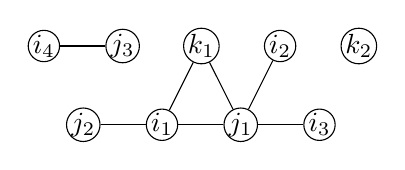
\begin{tikzpicture}
\node[draw,circle,inner sep=0pt] (I1) at (0,0) {$i_1$};
\node[draw,circle,inner sep=0pt] (J1) at (1,0) {$j_1$};
\node[draw,circle,inner sep=0pt] (K1) at (0.5,1) {$k_1$};
\node[draw,circle,inner sep=0pt] (J2) at (-1,0) {$j_2$};
\node[draw,circle,inner sep=0pt] (I2) at (1.5,1) {$i_2$};
\node[draw,circle,inner sep=0pt] (I3) at (2,0) {$i_3$};

\node[draw,circle,inner sep=0pt] (I4) at (-1.5,1) {$i_4$};
\node[draw,circle,inner sep=0pt] (J3) at (-0.5,1) {$j_3$};

\node[draw,circle,inner sep=0pt] (K2) at (2.5,1) {$k_2$};

\path[-] (I1) edge (J1) (J1) edge (K1) (K1) edge (I1);
\path[-] (J2) edge (I1) (J1) edge (I2) (J1) edge (I3);
\path[-] (I4) edge (J3); 
\end{tikzpicture}
\newline
PEO: $i_2$, $i_3$, $j_2$, $i_1$, $j_1$, $k_1$, $i_4$, $j_3$, $k_2$
\vspace*{10pt}

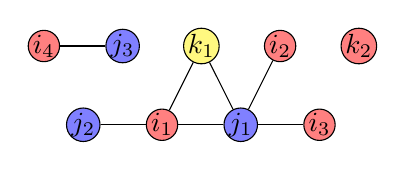
\begin{tikzpicture}
\node[draw,circle,inner sep=0pt,fill=red!50] (I1) at (0,0) {$i_1$};
\node[draw,circle,inner sep=0pt,fill=blue!50] (J1) at (1,0) {$j_1$};
\node[draw,circle,inner sep=0pt,fill=yellow!50] (K1) at (0.5,1) {$k_1$};
\node[draw,circle,inner sep=0pt,fill=blue!50] (J2) at (-1,0) {$j_2$};
\node[draw,circle,inner sep=0pt,fill=red!50] (I2) at (1.5,1) {$i_2$};
\node[draw,circle,inner sep=0pt,fill=red!50] (I3) at (2,0) {$i_3$};

\node[draw,circle,inner sep=0pt,fill=red!50] (I4) at (-1.5,1) {$i_4$};
\node[draw,circle,inner sep=0pt,fill=blue!50] (J3) at (-0.5,1) {$j_3$};

\node[draw,circle,inner sep=0pt,fill=red!50] (K2) at (2.5,1) {$k_2$};

\path[-] (I1) edge (J1) (J1) edge (K1) (K1) edge (I1);
\path[-] (J2) edge (I1) (J1) edge (I2) (J1) edge (I3);
\path[-] (I4) edge (J3); 
\end{tikzpicture}
\end{minipage}
&
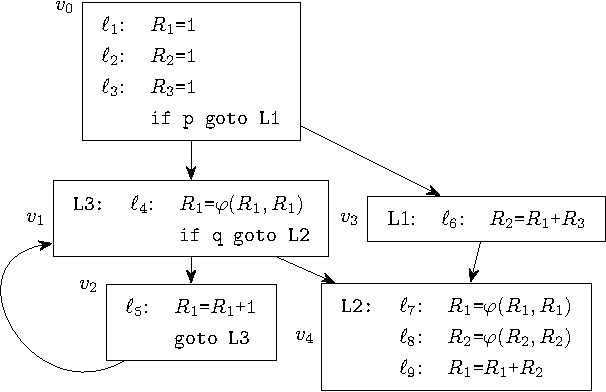
\includegraphics[width=\linewidth]{figs261127/SSA-example4-SSA-color-crop.pdf}
\end{tabularx}
\end{frame}

\subsection{$\varphi$関数消去}

\begin{frame}
\frametitle{レジスタ交換による$\varphi$関数の消去}
\greentext{\small 先の例：うまくレジスタ割当をすると$\varphi$関数はそのまま消去できた}

\vspace*{20pt}

\only<1>{
\begin{tabularx}{\linewidth}{m{.5\linewidth}m{.5\linewidth}}
    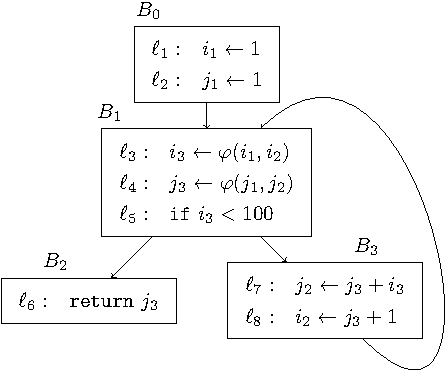
\includegraphics[width=\linewidth]{figs261127/SSA-regalloc-1-crop.pdf}
    &
    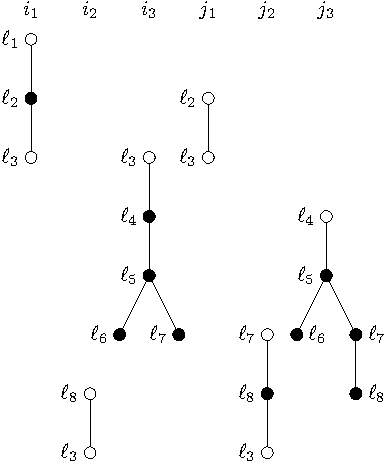
\includegraphics[scale=0.5]{figs261127/SSA-live-1-crop.pdf}
\end{tabularx}
}
\only<2->{
\begin{tabularx}{\linewidth}{m{.5\linewidth}m{.5\linewidth}}
    \multicolumn{1}{c}{干渉グラフ} & \multicolumn{1}{c}{レジスタ割当}\\
    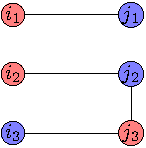
\includegraphics[scale=1]{figs261127/interfare-graph-1-crop.pdf}
    &
    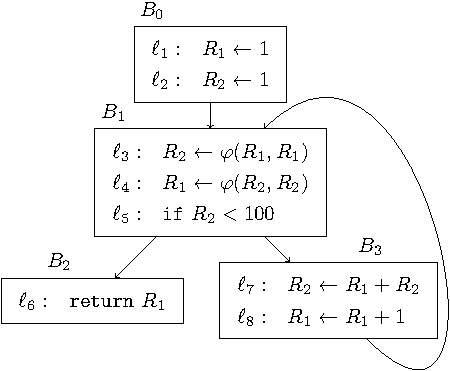
\includegraphics[scale=0.5]{figs261127/SSA-regalloc-1-res-crop.pdf}
\end{tabularx}  
}
\uncover<3>{
$\varphi$関数：ブロックの先頭にあり，変数ごとに独立＝並列代入\\
この場合，$\texttt{swap}\ R_1,R_2$で実現
}
\end{frame}

\begin{frame}
\frametitle{代入による$\varphi$関数の消去の場合}
\only<1>{
\begin{tabularx}{\linewidth}{m{.5\linewidth}m{.5\linewidth}}
    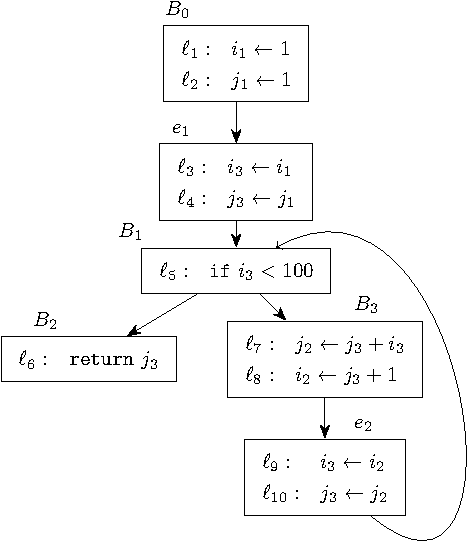
\includegraphics[width=\linewidth]{figs261127/SSA-regalloc-2-crop.pdf}
    &
    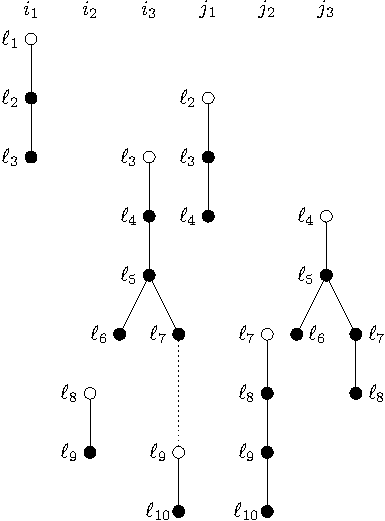
\includegraphics[scale=0.5]{figs261127/SSA-live-2-crop.pdf}
\end{tabularx}
}
\only<2->{
\begin{tabularx}{\linewidth}{m{.5\linewidth}m{.5\linewidth}}
    \multicolumn{1}{c}{干渉グラフ} & \multicolumn{1}{c}{レジスタ割当}\\
    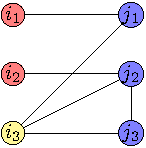
\includegraphics[scale=1]{figs261127/interfare-graph-2-crop.pdf}
    &
    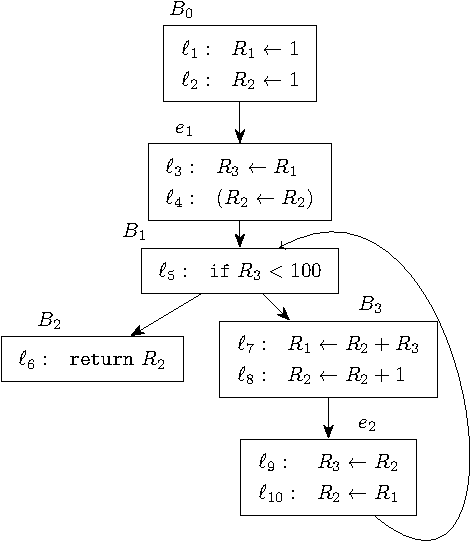
\includegraphics[scale=0.5]{figs261127/SSA-regalloc-2-res-crop.pdf}
\end{tabularx}  
}
\uncover<3>{\greentext{
    \small
    この場合は干渉グラフは弦グラフになるが，最大クリークサイズは３\\
    ３色で彩色されるので，レジスタは３必要}\\
    \redtext{\small 一般には弦グラフになることが保証されない}
}
\end{frame}

\begin{frame}
\frametitle{その他のレジスタ割り当ての問題}
\begin{list}{}{}
    \item[レジスタスピル最適化：] 実際に必要なレジスタ数が利用できるレジスタ数を上回る場合，メモリに一時的に Store する．必要になると load する．この回数を最小にする．
    
    \greentext{今後，使われる見込みの少ない変数をspillに入れるようにする．最適化には探索が必要}

    \item[コアレッシング(Coalescing)最適化：]
    コピーされる変数を一つにまとめて数を減らして，最適化する．

    \greentext{干渉も融合されるため，Spillが増加する可能性がある．} 
\end{list}

以上の動作を含めると，SSA形式においてもレジスタ割り当て問題自体はNP完全であることに変わりはない．
\end{frame}


\begin{frame}
 \frametitle{定期試験および評価}

 \begin{list}%
  {$\bullet$} %default label
  {} %formatting parameter
  \item 定期試験：12月1日(火) 14:45--16:15\\
  \qquad \underline{\bf 295演習室}(持込不可)\\
	・{\small (病欠など)追試験については，可能な限り事前に連絡の上で，
  所定の手続で情報学部教務へ申請すること．
  (手続きなしに追試験は実施しません．)}

詳細は，学部「在学生向け掲示板」(No.2223)を参照すること

  \item 評価：定期試験(50\%)+演習問題$\cdot$演習課題レポート(50\%)\\
	\greentext{状況に応じて比率は変更することがある．ただし，比率の
	変更が合否に直接関わることがないように配慮する．}
  \item 評価後にボーダーラインの成績の場合，追加課題を出すことがあるので，
  TACTのお知らせと全学メールに注意すること．
	 \end{list}
\end{frame}



\end{document}
